\documentclass[11pt]{amsart}
\usepackage[T1]{fontenc}
\usepackage{lmodern}
\usepackage{amsmath,amssymb,amsthm,mathtools}
\usepackage{booktabs}
\usepackage[margin=1.15in]{geometry}
\usepackage{pgfplots}
\pgfplotsset{compat=1.17}
\usepackage{xurl}
\usepackage[colorlinks=true,linkcolor=blue!50!black,citecolor=blue!50!black,urlcolor=blue!50!black,pdftitle={Collision primes of J0(23)},pdfauthor={Jesus Vilela Jato}]{hyperref}

\newtheorem{theorem}{Theorem}[section]
\newtheorem{lemma}[theorem]{Lemma}
\newtheorem{proposition}[theorem]{Proposition}
\newtheorem{corollary}[theorem]{Corollary}
\newtheorem{conjecture}[theorem]{Conjecture}
\theoremstyle{definition}
\newtheorem{definition}[theorem]{Definition}
\theoremstyle{remark}
\newtheorem{remark}[theorem]{Remark}

\newcommand{\Q}{\mathbb{Q}}
\newcommand{\Z}{\mathbb{Z}}
\newcommand{\F}{\mathbb{F}}
\newcommand{\cO}{\mathcal{O}}
\newcommand{\T}{\mathbb{T}}
\newcommand{\GL}{\mathrm{GL}}
\newcommand{\SL}{\mathrm{SL}}
\newcommand{\Gal}{\mathrm{Gal}}
\newcommand{\SU}{\mathrm{SU}}
\newcommand{\Frob}{\mathrm{Frob}}
\newcommand{\tr}{\operatorname{tr}}

\title[Collision primes of $J_0(23)$]{Collision primes of $J_0(23)$: forced congruences, exceptional local factors, and a pre-registered test of the Murty--Van Hirtum constant}

\author{Jes\'us Vilela Jato}
\address{Independent researcher, Madrid, Spain}

\date{November 23, 2026}

\subjclass[2020]{11F33, 11F80, 11G10, 11N05, 11Y35}
\keywords{Lang--Trotter conjecture, Frobenius traces, real multiplication, Eisenstein ideal, icosahedral representations, $J_0(23)$}

\begin{document}

\begin{abstract}
Let $f$ be the newform of weight $2$ and level $23$, with coefficient field $\Q(\sqrt5)$. Call a prime $p\neq 2,23$ a \emph{collision prime} if $a_p(f)\in\Z$, that is, if the two Galois-conjugate Hecke eigenvalues coincide. We prove that at a collision prime $a_p(f)\equiv p+1\pmod{11}$, and that $a_p(f)\bmod 2$ is determined by the class of $p$ in the Hilbert class field of $\Q(\sqrt{-23})$. Hence $a_p(f)\bmod 22$ is a function of $p$ alone. We also record a mod-$4$ lemma and state a mod-$4$ conjecture, supported by $1.19\times10^6$ cases without exception.

On the quantitative side, we replace the empirically fitted exceptional local factors in Van Hirtum's heuristic for $\#\{p\le x: a_p(f)\in\Q\}$ by factors computed from explicit models of the Galois image: an Eisenstein factor at $11$ and an icosahedral factor at $3$. The factor at $2$ remains empirical. A model fixed in advance using the generic factor at $3$ was refuted ($z=+8.4$). The corrected model was frozen before computing the range $(2\cdot10^7,6\cdot10^7]$, and there predicted $914.9$ collisions against $909$ observed. The asymptotic constant obtained is $c\approx4.864$. We argue that the $\approx10\%$ gap between Van Hirtum's fitted ($5.490$) and predicted ($4.982$) constants for this form is explained by the second-order term of $\sum_{p\le x}p^{-1/2}$. All data ($3{,}562{,}113$ primes), code and frozen pre-registrations are public.
\end{abstract}

\maketitle

\section{Introduction}

Let $f=\sum a_nq^n\in S_2(\Gamma_0(23))$ be a newform. Its Hecke field is $K=\Q(\sqrt5)$; write $\phi=(1+\sqrt5)/2$ and $\cO=\Z[\phi]$. The Galois conjugate $f^\sigma$ is the other newform, and $J_0(23)$ is a simple abelian surface with real multiplication by $\cO$ over $\Q$ \cite{Hashimoto,LMFDB}. Write
\[
a_p(f)=u_p+v_p\phi,\qquad u_p,v_p\in\Z .
\]

\begin{definition}
A prime $p\neq2,23$ is a \emph{collision prime} if $a_p(f)=a_p(f^\sigma)$, i.e.\ $v_p=0$, i.e.\ $a_p(f)\in\Z$.
\end{definition}

The first collision primes are $13,19,29,43,109,223,229,271,463,673,\dots$. Since $f$ has no inner twist, Ribet's theorems \cite{Ribet} imply that collision primes have density zero. A conjecture of V.~K.~Murty \cite{Murty}, extending Lang and Trotter \cite{LT}, in the form stated by Van Hirtum \cite[Conj.~1.1]{VH}, predicts
\begin{equation}\label{eq:murty}
\#\{p\le x:\ a_p(f)\in\Q\}\ \sim\ c_f\,\frac{\sqrt{x}}{\log x},
\qquad c_f=\frac{16\sqrt{D}\,\widehat F_f}{3\pi^2},
\end{equation}
where $D=5$ and $\widehat F_f=\lim_m F_m$ is a limit of local divisibility densities. Van Hirtum computed the unramified large-image factors and tested level $23$ up to $10^8$; for the ramified and exceptional primes he used empirical frequencies \cite[\S7]{VH}. Amri \cite[App.~A]{Amri} has recently proved that $\widehat F_f$ exists and is positive in general, and that it factors as a \emph{joint} exceptional factor times the unramified factors. No explicit exceptional factors for a specific form are computed there.

This note does three things for level $23$.
\begin{enumerate}
\item Section~\ref{sec:congr}: collision primes satisfy forced congruences modulo $11$ and $2$ (Theorem~\ref{thm:A}), together with a mod-$4$ lemma and a mod-$4$ conjecture.
\item Section~\ref{sec:local}: the exceptional factors at $3$, $11$ and $5$ are derived from explicit models of the Galois image by exact counting, instead of being fitted.
\item Section~\ref{sec:test}: the resulting constant is tested against $3{,}562{,}113$ primes, using predictions frozen (by SHA-256 hash) before the data were computed. This includes an honest record of a failed first model.
\end{enumerate}
We claim no new theorem of depth. Theorem~\ref{thm:A} is a short consequence of Mazur's work and of the structure of $J_0(23)[2]$; we have not found it stated in the literature. The infinitude of collision primes remains open.

\subsection*{Data and code}
Everything is available at \url{https://github.com/Dojo-1/J0-23-collision-primes}: code, ten regression tests, the values $(u_p,v_p)$ for all primes up to $6\cdot10^7$, and both pre-registrations with their hashes. This work grew out of round R14 of the Bolyai Research Atlas \cite{Atlas}.

\section{Computing the coefficients}\label{sec:coeffs}

Let $\theta_1=\sum_{x,y}q^{x^2+xy+6y^2}$ and $\theta_2=\sum_{x,y}q^{2x^2+xy+3y^2}$ be the theta series of the two reduced forms of discriminant $-23$ (up to $GL_2(\Z)$). They have weight $1$ and character $\left(\frac{-23}{\cdot}\right)$. Put
\[
B=\tfrac12(\theta_1-\theta_2)=\eta(z)\eta(23z)=q-q^2-q^3+q^6+q^8-q^{13}-\cdots .
\]

\begin{proposition}\label{prop:eta}
In the normalisation $a_p(f)=u_p+v_p\phi$ with $\phi^2=\phi+1$,
\[
\sum_n v_nq^n=\eta(z)^2\eta(23z)^2,\qquad \sum_n u_nq^n=\theta_2\,\eta(z)\eta(23z).
\]
\end{proposition}

\begin{proof}
The three products $\theta_1^2,\theta_1\theta_2,\theta_2^2$ lie in $M_2(\Gamma_0(23))$, which has dimension $3$. Comparing $q$-expansions, both identities are linear relations in this space. By Sturm's bound \cite{Sturm} it suffices to check coefficients up to $n=2\cdot24/12=4$. We checked them up to $n=10^4$ against PARI/GP's \texttt{mfcoefs} \cite{PARI}.
\end{proof}

Proposition~\ref{prop:eta} reduces the computation of $(u_p,v_p)$ for $p\le N$ to two FFT convolutions of length $O(N)$. For $N=6\cdot10^7$ the largest rounding residual at a prime was below $4\cdot10^{-11}$. As an independent check, the resulting Euler factors agree with point counts on the genus-$2$ model $y^2+(x^3+x+1)y=-x^5$ of $X_0(23)$ (PARI's \texttt{hyperellcharpoly}) at $468$ primes below $12{,}000$, with no mismatch.

\section{Forced congruences}\label{sec:congr}

We use the following standard inputs:
\begin{itemize}
\item[(I1)] (Mazur \cite{Mazur}) For prime level $N$, the Eisenstein ideal $I\subset\T$ is generated by $T_\ell-1-\ell$ ($\ell\neq N$) and $1+w_N$, and $\T/I\cong\Z/n\Z$ with $n=\mathrm{num}\big((N-1)/12\big)$. For $N=23$, $n=11$.
\item[(I2)] $\operatorname{End}(J_0(23))=\cO$ \cite{Hashimoto,LMFDB}. Since $T_2$ satisfies $x^2+x-1=0$, we get $\cO=\Z[T_2]\subseteq\T\subseteq\cO$, so $\T=\cO$.
\item[(I3)] (Eichler--Shimura \cite{Shimura}) For $\ell\neq p$, the Tate module $T_\ell J_0(23)$ is free of rank $2$ over $\cO\otimes\Z_\ell$, and $\Frob_p$ acts on it with trace $T_p$ and determinant $p$.
\end{itemize}

Let $H$ be the Hilbert class field of $\Q(\sqrt{-23})$, the splitting field of $x^3-x-1$, with $\Gal(H/\Q)\cong S_3$. A prime $p\neq23$ splits completely in $H$ iff $p=x^2+xy+6y^2$. It has Frobenius of order $3$ iff $p=2x^2+xy+3y^2$, and Frobenius of order $2$ iff $\left(\frac{-23}{p}\right)=-1$.

\begin{lemma}\label{lem:J2}
$\Q(J_0(23)[2])=H$.
\end{lemma}

\begin{proof}
Completing the square in $y^2+(x^3+x+1)y=-x^5$ gives $(2y+x^3+x+1)^2=F(x)$ with
\[
F(x)=(x^3+x+1)^2-4x^5=(x^3-2x^2-3x-1)(x^3-2x^2+x-1).
\]
Both cubic factors are irreducible over $\Q$ (no rational roots) and have discriminant $-23$. The cubic field of discriminant $-23$ is unique up to isomorphism, so both factors split in $H$, and the splitting field of $F$ is $H$. For a genus-$2$ curve $y^2=F(x)$ with $\deg F=6$, the field generated by the $2$-torsion of the Jacobian is the splitting field of $F$. (Schoof uses another model of the same curve \cite{Schoof}.)
\end{proof}

\begin{theorem}\label{thm:A}
Let $p\neq2,23$ be a collision prime and $a=a_p(f)\in\Z$. Then
\[
a\equiv p+1\pmod{11},\qquad
a\equiv\begin{cases}1,&p=2x^2+xy+3y^2,\\ 0,&\text{otherwise,}\end{cases}\pmod 2.
\]
In particular $a\bmod22$ is determined by $p$, and $a_p(f)=0$ implies $p\equiv10\pmod{11}$.
\end{theorem}

\begin{proof}
\emph{Mod $11$.} By (I2), $T_p=a\in\Z\subset\T$. By (I1), $a-1-p\in I\cap\Z$, and $I\cap\Z=11\Z$ because $\Z\to\T/I\cong\Z/11$ is surjective.

\emph{Mod $2$.} By (I3) and Lemma~\ref{lem:J2}, $G_\Q$ acts on $J[2]\cong\F_4^2$ through $\Gal(H/\Q)\cong S_3$, $\F_4$-linearly ($\cO/2\cong\F_4$, since $2$ is inert in $K$), with determinant the mod-$2$ cyclotomic character, which is trivial. The image is therefore a subgroup of $\SL_2(\F_4)\cong A_5$ of order dividing $6$. In $\SL_2(\F_4)$, elements of order $1$ or $2$ have trace $0$, elements of order $3$ have trace $1$, and only elements of order $5$ have trace in $\F_4\setminus\F_2$. Hence $T_p\bmod2\cO\in\F_2$, and it equals $1$ exactly when $\Frob_p$ has order $3$ in $\Gal(H/\Q)$ (the action is faithful because $H=\Q(J[2])$). At a collision prime $T_p=a$, so $a\bmod2$ is this trace.
\end{proof}

\begin{corollary}\label{cor:even}
For every $p\neq2,23$, $v_p$ is even.
\end{corollary}

\begin{proof}
$T_p\bmod 2\cO\in\F_2$ means $\phi$-coordinate $v_p\equiv0\pmod2$. An elementary second proof: by Proposition~\ref{prop:eta}, $v_p=\sum_{m=1}^{p-1}b_mb_{p-m}$ where $B=\sum b_nq^n$. For odd $p$ the terms pair off under $m\leftrightarrow p-m$ with $m\neq p-m$.
\end{proof}

\begin{lemma}\label{lem:R1}
If $p=x^2+xy+6y^2$, then $T_p\equiv1+p\pmod{4\cO}$. In particular $4\mid v_p$.
\end{lemma}

\begin{proof}
$\Frob_p$ acts trivially on $J[2]$, so on $T_2J$ it equals $1+2X$ with $X\in M_2(\cO_2)$. Then $T_p=2+2\tr X$ and $p=\det(1+2X)=1+2\tr X+4\det X$. Hence $1+p-T_p=4\det X$.
\end{proof}

\begin{conjecture}\label{conj:R2}
If $p=2x^2+xy+3y^2$, then $v_p\equiv p-1\pmod4$.
\end{conjecture}

Conjecture~\ref{conj:R2} is not a formal consequence of the mod-$2$ structure. Write $\Frob_p=A+2\phi B$ with $A,B\in M_2(\Z_2)$ in a basis where the mod-$2$ image is $\F_2$-rational. Then $v_p=2\tr B$, while $p\equiv\det A\pmod 4$, and nothing above links $\tr B\bmod2$ to $\det A\bmod4$. So Conjecture~\ref{conj:R2} is a constraint on the $2$-adic image itself. It plausibly follows from Schoof's analysis of the $2$-divisible group of $J_0(23)$ \cite{Schoof}, which we have not carried out.

For inert $p$, $v_p\bmod4$ is equidistributed in our data ($0.4998$ vs.\ $0.5002$).

\begin{remark}[Verification]
For all $3{,}562{,}113$ primes $3\le p\le6\cdot10^7$, $p\neq23$, the following hold with no exceptions: Theorem~\ref{thm:A} ($2{,}386$ collision primes), Corollary~\ref{cor:even}, the congruence $a_p(f)\equiv1+p\pmod{(11,\phi-4)}$, Lemma~\ref{lem:R1} ($593{,}491$ primes) and Conjecture~\ref{conj:R2} ($1{,}187{,}172$ primes). The only primes up to $6\cdot10^7$ with $a_p(f)=0$ are $43$, $109$ and $1033$, all $\equiv10\pmod{11}$.
\end{remark}

\section{Exceptional local factors from image models}\label{sec:local}

Following \cite{VH,Amri}, for a prime $\ell$ set
\[
F_\ell^{(k)}=\ell^k\cdot\Pr\big[\tr g\in\Z/\ell^k\big],
\]
where $g$ is Haar-distributed on the image of $G_\Q$ in $\GL_2(\cO/\ell^k)$. Then $F_\ell=\lim_kF_\ell^{(k)}$, and empirically $F_\ell^{(k)}$ equals $\ell^k$ times the frequency of primes with $\ell^k\mid v_p$. Van Hirtum's closed forms \cite[Props.~5.5--5.8]{VH} hold for unramified $\ell$ with image $\{g:\det g\in\Z_\ell^\times\}$. Our exact enumeration reproduces them: for example $F_3^{(1)}=87/80$, $F_3^{(2)}=263/240$, with limit $1.096875$.

\subsection{\texorpdfstring{$\ell=11$}{l=11}: Eisenstein}
$11$ splits in $K$. At the Eisenstein prime $\mathfrak P=(11,\phi-4)$, Mazur shows (for prime level with $n$ odd) that $J[\mathfrak P]$ is the direct sum of the cuspidal group $\Z/11$ and the Shimura subgroup $\mu_{11}$ \cite{Mazur}. So $\bar\rho_{\mathfrak P}\simeq1\oplus\chi_{11}$, and we take the $\mathfrak P$-adic image to be the full preimage of the diagonal $\{\mathrm{diag}(1,*)\}$. At the other prime above $11$ we assume full image, and the two components share their determinant. Exact counting gives
\[
F_{11}^{(1)}=1.09083,\quad F_{11}^{(2)}=1.09917,\quad F_{11}^{(3)}=1.09924 .
\]
The empirical values are $1.0948$ and $1.1083$ (standard errors about $0.01$). A Borel-type model, which is inconsistent with the split kernel, would give $F_{11}^{(2)}=1.0916$. For comparison, the generic split factor at $11$ is $1.0076$.

\subsection{\texorpdfstring{$\ell=3$}{l=3}: icosahedral}
The literature records that the mod-$3$ representation of $f$ has projective image $A_5$ \cite{BD}. Our data show exactly which coset structure occurs. For $p\equiv1\pmod3$, $T_p\bmod3\in\F_9$ never equals $\pm\phi^2$; for $p\equiv2\pmod3$, it never equals $\pm1$. The remaining frequencies are $0.250$, $0.175$ and $0.100$. These coincide to three decimals with the trace distribution of $G_3=\langle i\rangle\cdot2.A_5\subset\GL_2(\F_9)$, where $2.A_5\cong\SL_2(\F_5)$ is the binary icosahedral group embedded in $\SL_2(\F_9)$, $i=\phi^2$ and $i^2=-1$. In $2.A_5$, the trace is $0$ on $30$ of $120$ elements, $\pm1$ on $21$ each, and each of the four values $(\pm1\pm\sqrt5)/2$ on $12$. Taking the full preimage of $G_3$ gives
\[
F_3^{(1)}=\tfrac{51}{40},\quad F_3^{(2)}=\tfrac{53}{40},\qquad F_3\approx1.332,
\]
compared with the empirical values $1.2750$, $1.3258$, $1.3328$ and $1.3333$ for $k=1,\dots,4$.

\subsection{\texorpdfstring{$\ell=5$ and $\ell=2$}{l=5 and l=2}}
$5$ ramifies in $K$. With full image, $F_5^{(1)}=31/30$ and $F_5^{(2)}=388/375$, so $F_5\approx1.0347$; the empirical values are $1.0304$ and $1.0259$.

At $2$, Theorem~\ref{thm:A} puts the mod-$2$ image inside $\GL_2(\F_2)$. The full preimage of that image gives $F_2^{(k)}=2,\tfrac73,\tfrac{29}{12},\tfrac{39}{16}\to\tfrac{22}9$. The data give $2,\ 2.332,\ 2.501,\ 2.542,\ 2.554$. The model therefore fails at $k\ge3$, as Conjecture~\ref{conj:R2} predicts: the full preimage gives $\Pr[4\mid v_p]=7/12$ for both classes $p\bmod 4$, whereas the data give $3/4$ for $p\equiv1$ and $5/12$ for $p\equiv3$. We therefore use the empirical value $F_2=2.554$ and leave the $2$-adic image open.

\subsection{Independence}
The model below multiplies the exceptional factors, which assumes independence across $\ell$; Amri's joint factor \cite{Amri} allows for dependence. The one entanglement visible here is between the $2$-adic and $23$-adic images, through $\sqrt{-23}\in H\cap\Q(\zeta_{23})$. It changes the product by less than $2\cdot10^{-4}$, because the $23$-adic factor depends on $\left(\frac{p}{23}\right)$ only at relative order $2/23^3\approx1.6\cdot10^{-4}$.

\section{A pre-registered test}\label{sec:test}

The archimedean factor comes from the Sato--Tate group $\SU(2)\times\SU(2)$: $\Pr[v_p=0]\approx\frac{8\sqrt5}{3\pi^2}\widehat F\,p^{-1/2}$ \cite[Lemma~4.5]{VH}. We predict
\[
N(x)=\#\{p\le x:\ v_p=0\}\ \approx\ \frac{8\sqrt5\,\widehat F}{3\pi^2}\sum_{3\le p\le x,\ p\neq23}p^{-1/2}.
\]

\textbf{Model M1} was frozen before any computation beyond $p\le101$ (SHA-256 \texttt{f3d823ab\ldots}). It used $F_2=22/9$, $F_{11}$ as above, and the \emph{generic} $F_3$, giving $\widehat F=3.1729$. It was refuted: at $x=2\cdot10^7$ it predicted $1187.9$ against $1477$ observed ($z=+8.4$). Its pre-registered local tests located the failure at $\ell=3$ ($z=+147$) and at $\ell=2$, $k\ge3$, while $\ell=5$ and $\ell=11$ passed. This is how the icosahedral structure above was found.

\textbf{Model M2} is exploratory, being chosen after M1 failed. It uses the icosahedral $F_3=1.332$ and the empirical $F_2=2.554$. The latter is estimated from local frequencies over all primes, not from collision counts. This gives $\widehat F=4.026$ and $c_f=16\sqrt5\widehat F/(3\pi^2)=4.864$. M2 was frozen (SHA-256 \texttt{c71a78e4\ldots}) before the range $(2\cdot10^7,6\cdot10^7]$ was computed.

\begin{table}[h]
\centering
\begin{tabular}{@{}lrrrr@{}}
\toprule
held-out range & observed & M2 & $z_{\rm M2}$ & $z_{\rm M1}$\\
\midrule
$(2\cdot10^7,4\cdot10^7]$ & 504 & 524.6 & $-0.90$ & $+4.45$\\
$(4\cdot10^7,6\cdot10^7]$ & 405 & 390.3 & $+0.75$ & $+5.55$\\
$(2\cdot10^7,6\cdot10^7]$ & 909 & 914.9 & $-0.19$ & $+7.00$\\
\bottomrule
\end{tabular}
\caption{Held-out test. $z=(\text{obs}-\text{pred})/\sqrt{\text{pred}}$.}
\end{table}

\begin{figure}[h]
\centering
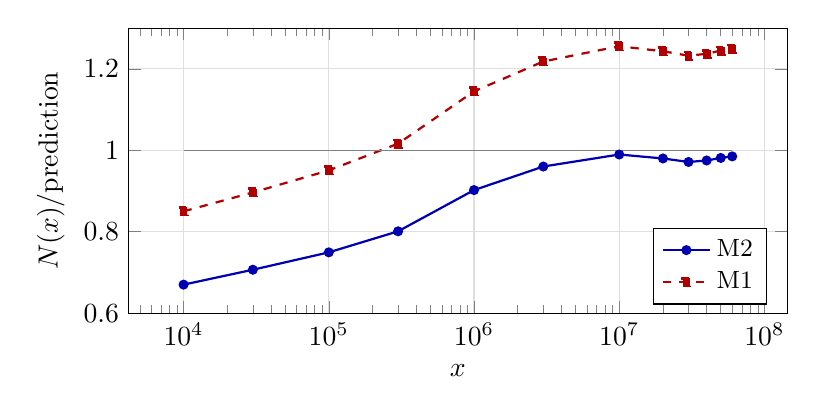
\begin{tikzpicture}
\begin{axis}[width=0.82\textwidth,height=5.2cm,xmode=log,xlabel={$x$},ylabel={$N(x)/\text{prediction}$},
  ymin=0.6,ymax=1.3,legend pos=south east,legend style={font=\small},grid=major,grid style={gray!25}]
\addplot[thick,mark=*,mark size=1.4pt,blue!70!black] coordinates {(1e4,0.6700)(3e4,0.7066)(1e5,0.7493)(3e5,0.8010)(1e6,0.9023)(3e6,0.9602)(1e7,0.9897)(2e7,0.9800)(3e7,0.9714)(4e7,0.9750)(5e7,0.9813)(6e7,0.9851)};
\addplot[thick,dashed,mark=square*,mark size=1.4pt,red!70!black] coordinates {(1e4,0.8501)(3e4,0.8965)(1e5,0.9507)(3e5,1.0164)(1e6,1.1448)(3e6,1.2183)(1e7,1.2557)(2e7,1.2434)(3e7,1.2325)(4e7,1.2371)(5e7,1.2451)(6e7,1.2499)};
\addplot[gray,thin,domain=1e4:6e7] {1};
\legend{M2,M1}
\end{axis}
\end{tikzpicture}
\caption{Cumulative ratio of observed to predicted collision counts.}
\end{figure}

M2 overestimates at small $x$: the ratio is $0.75$ at $10^5$, $0.90$ at $10^6$, and $0.985$ to $0.99$ from $10^7$ on. The $p^{-1/2}$ approximation ignores finite-$p$ effects: the lattice of admissible $(a_p(f),a_p(f^\sigma))$, restricted by Theorem~\ref{thm:A} to classes mod $22$, sampled against the Sato--Tate density near the edges of the Hasse box. We have not modelled this.

\subsection{Van Hirtum's fitted constant}
For level $23$, Van Hirtum reports a predicted $\hat c=4.982$ (using empirical exceptional factors) and a constant $\tilde c=5.490$ fitted on $x\le10^8$, a ratio of $1.10$ \cite[Table~1]{VH}. Our $c_f=4.864$ is within $2.4\%$ of his prediction. The gap to the fitted value is not a missing factor: the quantity
\[
\Big(\sum_{p\le x}p^{-1/2}\Big)\Big/\Big(2\sqrt x/\log x\Big)
\]
equals $1.174$, $1.160$ and $1.146$ at $x=10^7$, $3\cdot10^7$ and $10^8$. A least-squares fit of $c\sqrt x/\log x$ to M2-expected counts at $50$ equally spaced points up to $10^8$ returns $5.60$, within $2\%$ of $5.490$. We did not re-inspect Van Hirtum's fitting window, so this explanation is inferred rather than verified. It suggests that comparisons with \eqref{eq:murty} should use $\sum p^{-1/2}$ rather than its leading asymptotic.

\section{Open problems}
\begin{enumerate}
\item Determine the $2$-adic image of $J_0(23)$. Prove Conjecture~\ref{conj:R2}, and check whether the full preimage of that image gives $F_2=2.554$ exactly.
\item Prove that the $3$-adic image is the full preimage of $\langle i\rangle\cdot2.A_5$, and compute $F_3$ exactly; the data and $k\le2$ suggest $F_3=4/3$.
\item Give a finite-$p$ refinement of the archimedean factor that explains the deficit at $x\le10^6$.
\item Formalise Theorem~\ref{thm:A} given (I1)--(I3); its arithmetic steps are finite.
\end{enumerate}

\subsection*{Use of AI}
The computations, the search for congruences and local-factor models, the proofs and the text were produced with substantial assistance from an AI system (Claude, Anthropic), working under the author's direction within the Bolyai Research Atlas project. Prompts and transcripts are available on request. Every numerical claim is reproducible from the public repository.

\begin{thebibliography}{99}

\bibitem{Amri} M.~A.~Amri, \emph{Effective Chebotarev--Sato--Tate distribution for abelian varieties with applications}, arXiv:2610.36464, 2026.

\bibitem{Atlas} Dojo-1, \emph{Bolyai Research Atlas}, \url{https://github.com/Dojo-1/Bolyai-Research-Atlas}, rounds R14--R14b, 2026.

\bibitem{BD} N.~Billerey and L.~V.~Dieulefait, \emph{Explicit large image theorems for modular forms}, J.\ London Math.\ Soc.\ (2) \textbf{89} (2014), 499--523; arXiv:1210.5428.

\bibitem{Hashimoto} K.~Hashimoto, \emph{On Brumer's family of RM-curves of genus two}, Tohoku Math.\ J.\ \textbf{52} (2000), 475--488.

\bibitem{LT} S.~Lang and H.~Trotter, \emph{Frobenius Distributions in $\GL_2$-Extensions}, Lecture Notes in Math.\ \textbf{504}, Springer, 1976.

\bibitem{LMFDB} The LMFDB Collaboration, \emph{The L-functions and modular forms database}, newform 23.2.a.a and genus-2 curve 529.a.529.1, \url{https://www.lmfdb.org}.

\bibitem{Mazur} B.~Mazur, \emph{Modular curves and the Eisenstein ideal}, Publ.\ Math.\ IH\'ES \textbf{47} (1977), 33--186.

\bibitem{Murty} V.~K.~Murty, \emph{Frobenius distributions and Galois representations}, in: Automorphic Forms, Automorphic Representations, and Arithmetic, Proc.\ Sympos.\ Pure Math.\ \textbf{66}, Part 1, Amer.\ Math.\ Soc., 1999, 193--211.

\bibitem{PARI} The PARI~Group, \emph{PARI/GP}, Univ.\ Bordeaux, \url{https://pari.math.u-bordeaux.fr}.

\bibitem{Ribet} K.~A.~Ribet, \emph{On $\ell$-adic representations attached to modular forms II}, Glasgow Math.\ J.\ \textbf{27} (1985), 185--194.

\bibitem{Schoof} R.~Schoof, \emph{On the modular curve $X_0(23)$}, in: Geometry and Arithmetic, EMS Ser.\ Congr.\ Rep., Eur.\ Math.\ Soc., 2012.

\bibitem{Shimura} G.~Shimura, \emph{Introduction to the Arithmetic Theory of Automorphic Functions}, Princeton Univ.\ Press, 1971.

\bibitem{Sturm} J.~Sturm, \emph{On the congruence of modular forms}, in: Number Theory (New York, 1984--85), Lecture Notes in Math.\ \textbf{1240}, Springer, 1987, 275--280.

\bibitem{VH} J.~Van Hirtum, \emph{On the distribution of Frobenius of weight $2$ eigenforms with quadratic coefficient field}, arXiv:1508.07206, 2018; see also his PhD thesis, \emph{Computational aspects of classical and Hilbert modular forms}, 2017.

\end{thebibliography}

\end{document}
